\section{Conceptos de Tránsito Vehicular}
El análisis del tráfico vehicular se fundamenta en la teoría del flujo vehicular, la cual describe la interacción entre vehículos, conductores e infraestructura. Las variables macroscópicas fundamentales son:

\textbf{Flujo ($q$):} Se define como la tasa a la cual los vehículos pasan por un punto específico de la vía durante un intervalo de tiempo. Se expresa comúnmente en vehículos por hora (veh/h) \cite{survey_prajapati2024,survey_haydari2022}.
\begin{equation}
    q = \frac{N}{T}
\end{equation}
Donde $N$ es el número de vehículos que pasan por el punto y $T$ es el intervalo de tiempo de observación.

\textbf{Densidad ($k$):} Representa el número de vehículos ocupando un segmento de longitud unitaria de la vía en un instante dado. Se expresa en vehículos por kilómetro (veh/km) \cite{survey_haydari2022}.

\textbf{Velocidad media espacial ($v_s$):} Es la media armónica de las velocidades de los vehículos que pasan por un punto. La relación fundamental del tráfico establece que \cite{survey_prajapati2024}:
\begin{equation}
    q = k \cdot v_s
\end{equation}
Donde $q$ es el flujo, $k$ es la densidad y $v_s$ es la velocidad media espacial.

\textbf{Diagrama Fundamental:} Describe la relación no lineal entre flujo y densidad. A medida que la densidad aumenta, el flujo crece hasta alcanzar una capacidad máxima ($q_{max}$), punto tras el cual el flujo colapsa debido a la congestión, entrando en un régimen inestable \cite{survey_haydari2022,review_noaeen2022}.

\textbf{Longitud de Cola:} Métrica crítica para el control semafórico, definida como el número de vehículos detenidos o avanzando a una velocidad inferior a un umbral en una aproximación. Minimizar esta variable es uno de los objetivos más frecuentes en los sistemas de control adaptativo \cite{review_rasheed2020,review_noaeen2022}.

\textbf{Fase Semafórica:} Intervalo de tiempo durante el cual un conjunto de movimientos vehiculares tiene derecho de paso mientras los movimientos conflictivos permanecen detenidos. Un ciclo semafórico completo se compone de una secuencia ordenada de estas fases \cite{survey_haydari2022}.

\section{SUMO: Características y Arquitectura}
La literatura reciente sobre control semafórico con aprendizaje por refuerzo valida de forma predominante sus propuestas en entornos de simulación microscópica y sobre benchmarks reproducibles antes de considerar una implementación en campo \cite{benchmark_ault2021,case_gokulan2020}. En esta tesis se emplea \textbf{SUMO (Simulation of Urban MObility)} como plataforma experimental para modelar una intersección urbana aislada y evaluar el agente bajo múltiples perfiles de demanda.

\textbf{Modelos de Seguimiento (Car-Following):} SUMO permite representar cada vehículo como un agente individual con parámetros físicos y de comportamiento. En esta configuración, la dinámica longitudinal se aproxima mediante reglas de seguimiento vehicular y distancias de seguridad entre un vehículo y su líder.
\begin{equation}
    v_{safe} = v_l(t) + \frac{g(t) - v_l(t) \tau}{ \frac{\bar{v}}{2b} + \tau }
\end{equation}
Donde $v_{safe}$ es la velocidad segura calculada, $v_l(t)$ es la velocidad del vehículo líder en el tiempo $t$, $g(t)$ es la brecha con el líder, $\tau$ es el tiempo de reacción del conductor, $b$ es la desaceleración máxima posible y $\bar{v}$ es la velocidad media promedio de los vehículos.

\textbf{TraCI (Traffic Control Interface):} Es el componente crucial para esta investigación. TraCI permite la comunicación bidireccional en tiempo real entre SUMO y un controlador externo. Esto permite al agente de RL:
\begin{enumerate}
    \item \textbf{Observar:} Leer estados de sensores simulados.
    \item \textbf{Actuar:} Modificar las fases de los semáforos dinámicamente en cada paso de simulación.
\end{enumerate}

\begin{figure}[H]
    \centering
    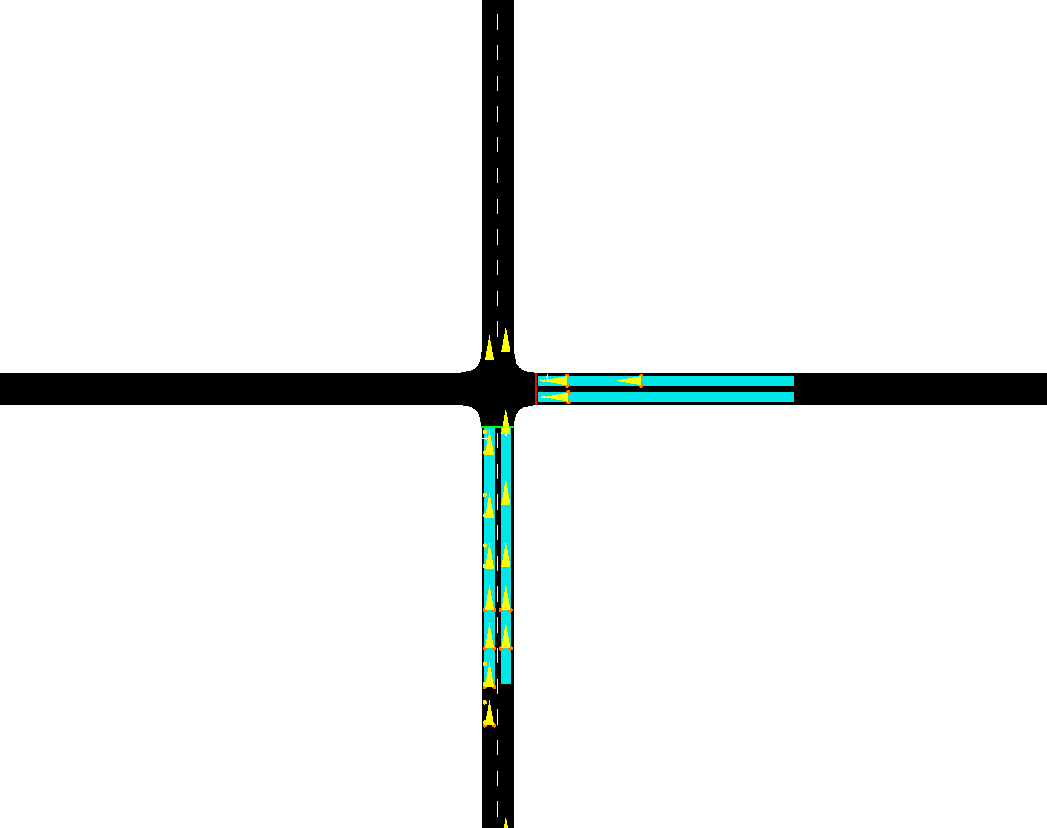
\includegraphics[width=0.8\textwidth]{images/Sumo-4vias.png}
    \caption{Visualización de la intersección simulada en SUMO, mostrando las 4 aproximaciones y la gestión semafórica.}
    \label{fig:sumo_4vias}
\end{figure}

\section{Fundamentos de Aprendizaje por Refuerzo (RL)}
El Aprendizaje por Refuerzo es un paradigma de aprendizaje automático donde un agente aprende a tomar decisiones secuenciales interactuando con un entorno. El problema se formaliza matemáticamente como un \textbf{Proceso de Decisión de Markov (MDP)}, definido por la tupla $(S, A, P, R, \gamma)$ \cite{rl_sutton2018}:

\begin{itemize}
    \item \textbf{$S$ (Espacio de Estados):} Conjunto de todas las configuraciones posibles del entorno.
    \item \textbf{$A$ (Espacio de Acciones):} Conjunto de decisiones disponibles para el agente.
    \item \textbf{$P(s'|s,a)$ (Probabilidad de Transición):} Dinámica del entorno que define la probabilidad de pasar al estado $s'$ dado el estado $s$ y la acción $a$.
    \item \textbf{$R(s,a)$ (Función de Recompensa):} Señal escalar que indica la calidad inmediata de la acción tomada.
    \item \textbf{$\gamma \in [0,1]$ (Factor de Descuento):} Determina la importancia de las recompensas futuras frente a las inmediatas.
\end{itemize}

El objetivo del agente es encontrar una política óptima $\pi^*(a|s)$ que maximice el retorno esperado $G_t$, definido como la suma descontada de recompensas futuras:
\begin{equation}
    G_t = \sum_{k=0}^{\infty} \gamma^k R_{t+k+1}
\end{equation}
Donde $G_t$ es el retorno esperado, $\gamma$ es el factor de descuento y $R_{t+k+1}$ es la recompensa recibida en el paso de tiempo $t+k+1$.

\section{Deep Reinforcement Learning y PPO}
El \textbf{Deep Reinforcement Learning (DRL)} integra redes neuronales profundas como aproximadores de funciones para estimar políticas $\pi_\theta(a|s)$ o valores $V_\theta(s)$ en espacios de estados de alta dimensión, superando las limitaciones del RL tabular.

\textbf{Proximal Policy Optimization (PPO):}
Dentro del control semafórico, PPO se ha consolidado como una alternativa práctica por su estabilidad de entrenamiento, su buen desempeño con observaciones continuas y su capacidad de generalización en escenarios aislados y multiagente \cite{compare_ouyang2024,ppo_karedla2025,haps_ppo2025}.

La función objetivo de PPO se define como:
\begin{equation}
    L^{CLIP}(\theta) = \hat{\mathbb{E}}_t [ \min(r_t(\theta)\hat{A}_t, \text{clip}(r_t(\theta), 1-\epsilon, 1+\epsilon)\hat{A}_t) ]
\end{equation}
Donde:
\begin{itemize}
    \item $\hat{\mathbb{E}}_t$ denota la esperanza empírica sobre los pasos de tiempo.
    \item $r_t(\theta)$ es el cociente de probabilidad entre la nueva y la vieja política.
    \item $\hat{A}_t$ es la estimación de la función de ventaja.
    \item $\epsilon$ es un hiperparámetro que limita el cambio de la política.
\end{itemize}

Este mecanismo favorece actualizaciones estables de la política, lo cual es especialmente valioso en entornos de control complejos como el tráfico urbano.
